\documentclass[conference]{IEEEtran}
\usepackage{cite}
\usepackage{amsmath,amssymb,amsfonts}
\usepackage{algorithmic}
\usepackage{graphicx}
\usepackage{textcomp}
\usepackage{xcolor}
\usepackage{hyperref}
\usepackage{tabularx}
\usepackage{float}

\title{Homework 2 Report - Artificial Neural Networks and Deep Learning}

\author{
Alberto Rota
    \IEEEauthorblockA{ \\
    \textit{Person Code: 10615751}\\
    \textit{Student Number: 964662} \\
    \href{mailto:alberto2.rota@mail.polimi.it}{alberto2.rota@mail.polimi.it}}
\and
Gabriele Santicchi 
    \IEEEauthorblockA{ \\
    \textit{Person Code: 10579046}\\
    \textit{Student Number: 969088}  \\
    \href{mailto:gabriele.santicchi@mail.polimi.it}{gabriele.santicchi@mail.polimi.it}}
\and
Giuseppe Venezia 
    \IEEEauthorblockA{ \\
    \textit{Person Code: 10622477 }\\
    \textit{Student Number: 968395}  \\
    \href{mailto:giuseppe.venezia@mail.polimi.it}{giuseppe.venezia@mail.polimi.it}}
}
\begin{document}

\maketitle

\section{Context}
    The goal of this competition is to build a forecasting model that  
    predicts the future trends of a multivariate time series by exploiting the past observations. The available dataset is
    composed of $7$ time-series, each composed of $68528$ samples. The hidden test sequence consists of 864 future values which have to be forecasted, providing the prediction for each time step. 

\section{Preparatory Tasks}

\subsection{Data Loading and Train-Validation Split}
    After having uploaded the dataset into the environment, the dataset has been divided into training and test sets, in order to use the entire training set for model selection and evaluation. \\

    
\subsection{Preprocessing}
    After the train-test splitting, the dataset has been inspected qualitatively in order to identify the presence of major issues with the data. 
    
    \begin{figure}[h]
        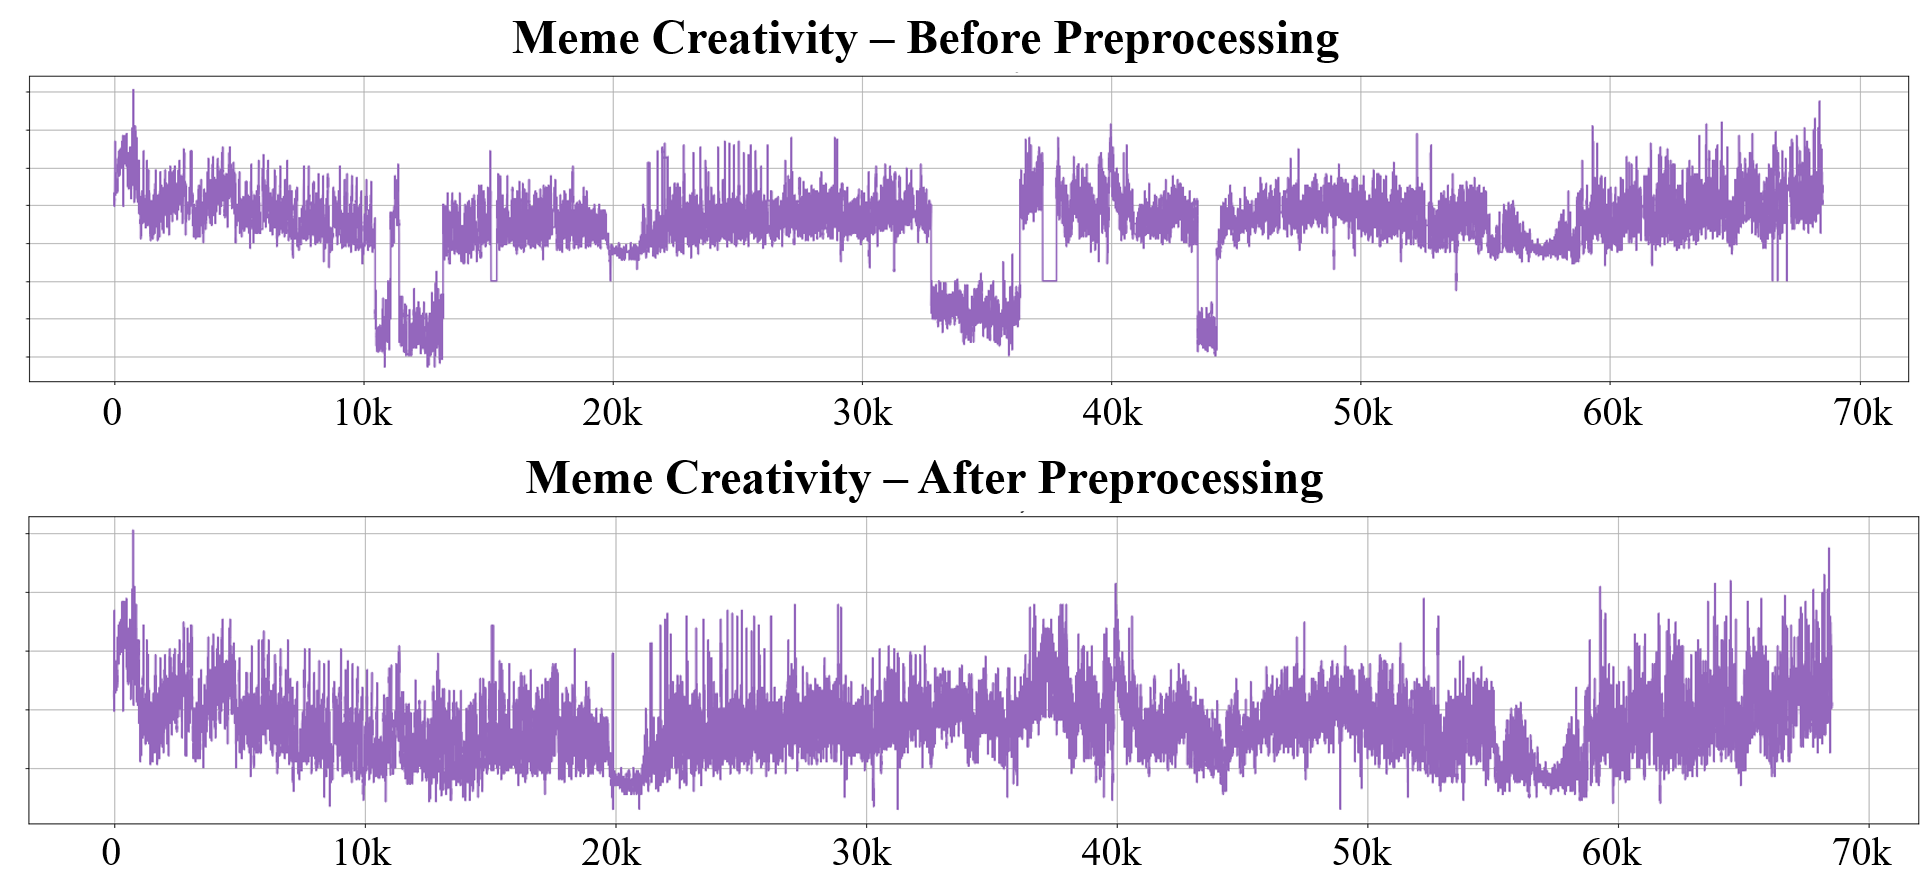
\includegraphics[width=\linewidth]{baseline_adjusted.png}
        \caption{'Meme Creativity' shows regions with abnormal loss of signal}
        \label{fig:baseline_adjusted}
    \end{figure}
    
    Most importantly, the time series are characterized by several flat regions of different length (Figure \ref{fig:baseline_adjusted});
    The same plot also highlights the presence of a large amount of samples whose mean is largely below the one of the overall time series.
    Both characteristics can be traced back to a loss of signal that can reduce the performance of the multivariate forecasting.
    
    These acknowledgments led to the an \textit{ad-hoc} implementation of two pre-processing functions. Briefly, the first one calculates the derivative of each variable, and if more than 5 consecutive samples in the  derivative are equal to zero, 
    the corresponding samples in the primitive time series are replaced by \textit{NaN} values. After that, the removed samples are interpolated with a symmetric replication, in order to avoid discontinuities and to replicate the trend of the data. Results of the symmetric on a flat window are shown in Figure \ref{fig:reflection_nan}.
    The second function gets as parameter a threshold (THR) value, and adds to each samples below THR the mean of the overall time series over THR. Results of this preprocessing step can be observed in Figure \ref{fig:baseline_adjusted}.
    Both of them have been applied as preprocessing steps in order to observe if the performance of the model would increase. 
    
   \begin{figure}[h]
        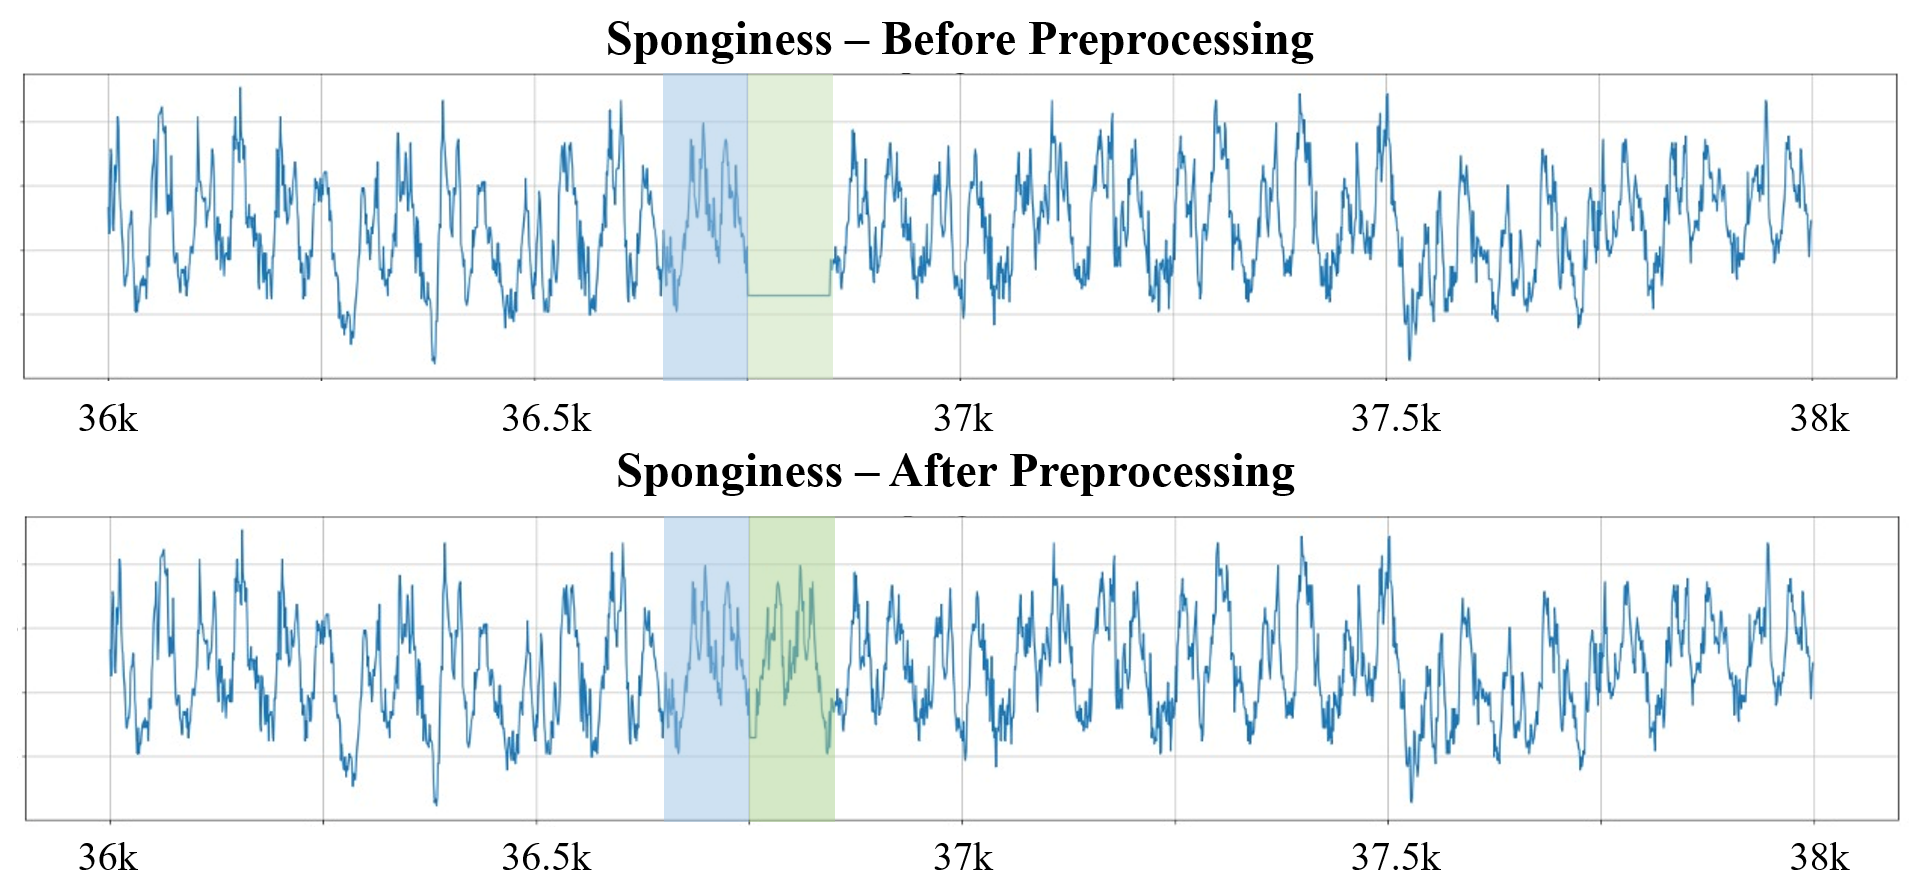
\includegraphics[width=\linewidth]{reflection_nan.png}
        \caption{Presence of a flat zone in the 'Sponginess' time-series.}
        \label{fig:reflection_nan}
    \end{figure}

\subsection{Normalization}
    A further step of the data preparation consists in a re-scaling of the data of all the time-series, by the means of a min-max approach. The re-scaling parameters have been computed for each time series of the training set and then used to normalize both the training and the test set. 
    
\subsection{Signal Windowing}
    Computing the prediction for the 864 samples in the future from the entire length of the available sequence would be unfeasible in terms of training time and inference time. Therefore, the training and test sets have been subdivided in a set of windows.
    From the results of a grid search, the stride and telescope hyperparameters have been set to 5 and 24 samples, respectively. 
    
    At the end of the train-test splitting and the windowing phase, the dataset consists of 12444 windows+labels dedicated to training and 931 dedicated to test. The test size is very limited on purpose since, for predicting the future of a time series, the most relevant information is located in the last samples. Indeed, the exclusion of a consistent number of the last windows in time from the training dataset will be negatively impactful on the model prediction.

\section{The Model}
    The width of the window that the model takes into consideration for the prediction is quite relevant on the prediction error: small windows may be best representative of the signal's detailed features, while with increasing width the window will also contain information about the signal baseline. Both of these factors have to be accounted by the model when inferencing the prediction, hence the width to be chosen must be of the optimal size to grasp both the short-term and long-term features. 

    The proposed model, instead, takes as input multiple windows at a time, each  one of different length: more specifically, from any set of  $N$ integer window widths $\textbf{w}=[w_1, w_2, ... w_N]$, the data is split in $N$ windows, as follows:
    $$Window_1 = Data[k : k+w_1]$$
    $$Window_2 = Data[k+w_1-w_2 : k+w_1]$$
    where $k$ is the initial window sample, dependent on the stride parameter. In general, the \textit{j-th} window is extracted as
    $$Window_j = Data[k+w_1-w_j : k+w_1]$$
    
    \begin{figure}[h!]
        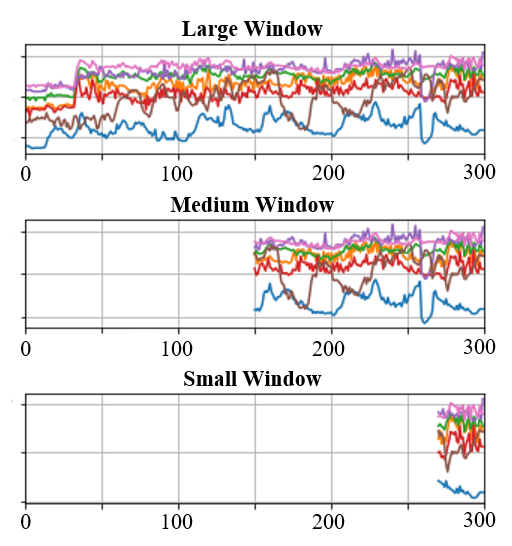
\includegraphics[width=0.45\textwidth]{windows.png}
        \caption{Multiple-length window splitting}
        \label{fig:windows}
    \end{figure}
    
    \begin{figure*}
        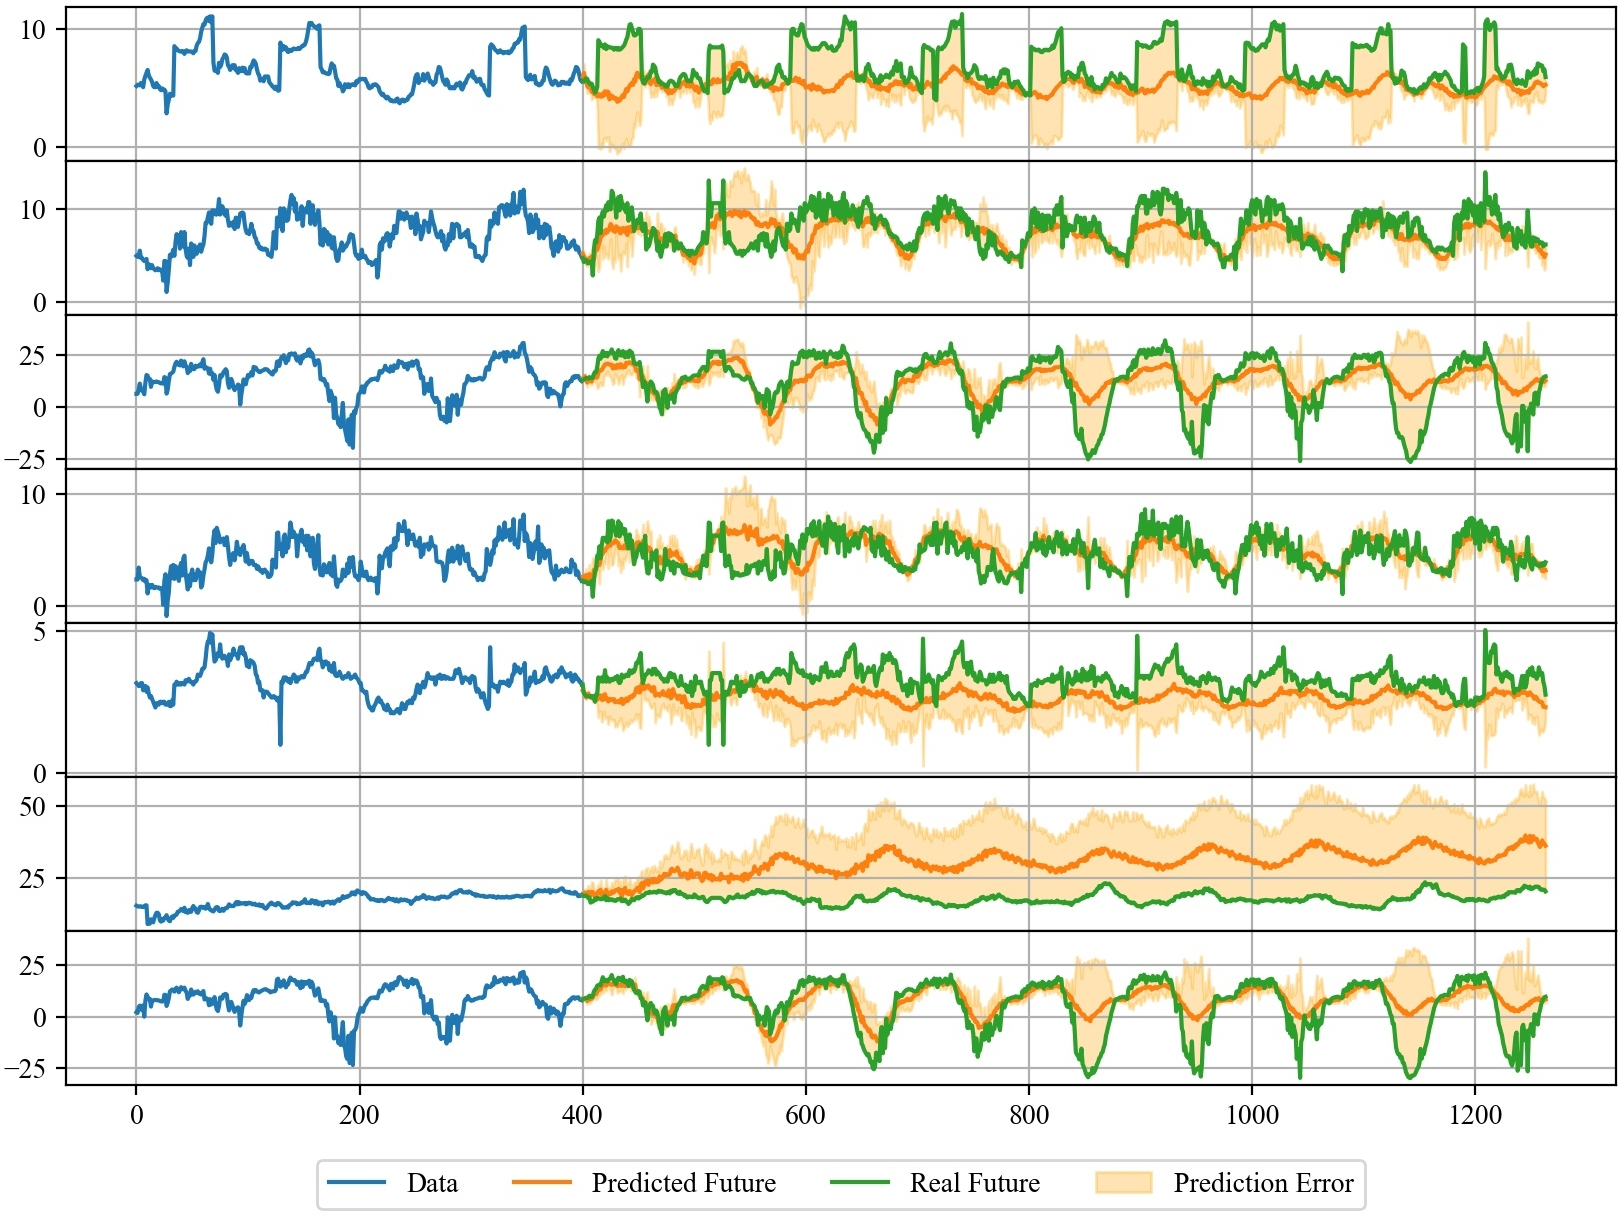
\includegraphics[width=\linewidth]{prediction.jpg}
        \caption{Prediction on the last \textit{864} samples.}
        \label{fig:prediction}
    \end{figure*}
    
    Figure \ref{fig:windows} shows an example of the multi-window splitting operation with the window width vector $\textbf{w}=[300,150,30]$.
    
    It was assessed that, when combining windows of different width in a single model, the optimal approach is to choose widths that span different orders of magnitude. More specifically, in this case, a grid search revealed that the optimal window sizes for the model (\textit{i.e.}, the one that results in the lowest validation loss) were of 400, 40 and 4 samples. It was later assessed that the 4-samples window was not in any way contributing to the model, and as a consequence the final splitting was performed on windows of 400 and 40 samples.   
    The proposed architecture is a recurrent neural network that combines 1D convolutional layers with Bidirectional Long Short-Term Memory cells. The architecture is mirrored on the two "tails" of the neural network, one for each window size, that converge at a concatenation layer where the features extracted at the different temporal scales are combined. The final prediction, of 24 samples, occurs after a couple of dense layers placed following the concatenation. All the 7 variables are predicted at once, in a multi-variate fashion: this assures that the prediction on any variable accounts for the features extracted from the other six, as their evident correlation suggests.
    
\section{Training}
    The model is trained minimizing a Mean Squared Error loss function by the means of the ADAM optimizer: similar performance have been obtained with MSE, MAE and RMSE. Batch size is set to 128, learning rate starts at $1\cdot 10^{-3}$ and is halved every time a plateau is reached by the validation loss. Overfitting is countered by an \textit{Early Stopping} callback and with the addition of \textit{Dropout} layers in the model. A first fitting phase of 50 epochs is performed on the training dataset, after which the model is evaluated in terms of performance and generalization capabilities: positively performing models are refined with a second fitting on the full dataset (training and testing) with a reduced learning rate and for a few epochs. It's important to denote that if this second training phase is carried out for too many epochs, it may cause the model to overfit.

\section{Results}
    The model performance has been assessed on the last \textit{864} samples of each time series and the prediction results are shown in Figure \ref{fig:prediction}.  
    The multi-window model is able to capture both the periodicity of the signals and the small variations through time. In particular, in the third and seventh time series, the model predicts accurately the small increase in the depth of the first four peaks. The best results have been obtained on the second and fourth signals, where the periodicity is predominant; the absence of evident variations among the series allows the model to perform well until the end of the range. 
    However, the forecast on the first and sixth time series got the maximum prediction error. As shown in Figure \ref{fig:prediction}, the model is not able to capture both rapid changes in the signal (see the peaks in the first one) and very low frequency trends in the 'Meme Creativity' time series. 
    To face these issues, some trials has been performed. First, a forecasting uni-variate model has been trained for these single time series to capture their specific high and low frequency features. Secondly, the weighted moving average of the 'Meme Creativity' has been added as a further time series to be predicted; with this approach the forecast on the signal would be the combination of the two predictions. 
    Unfortunately, both the trials performed worse than the original approach, so this latter has been chosen as the final one. 
    
    
    \begin{figure*}[h!]
        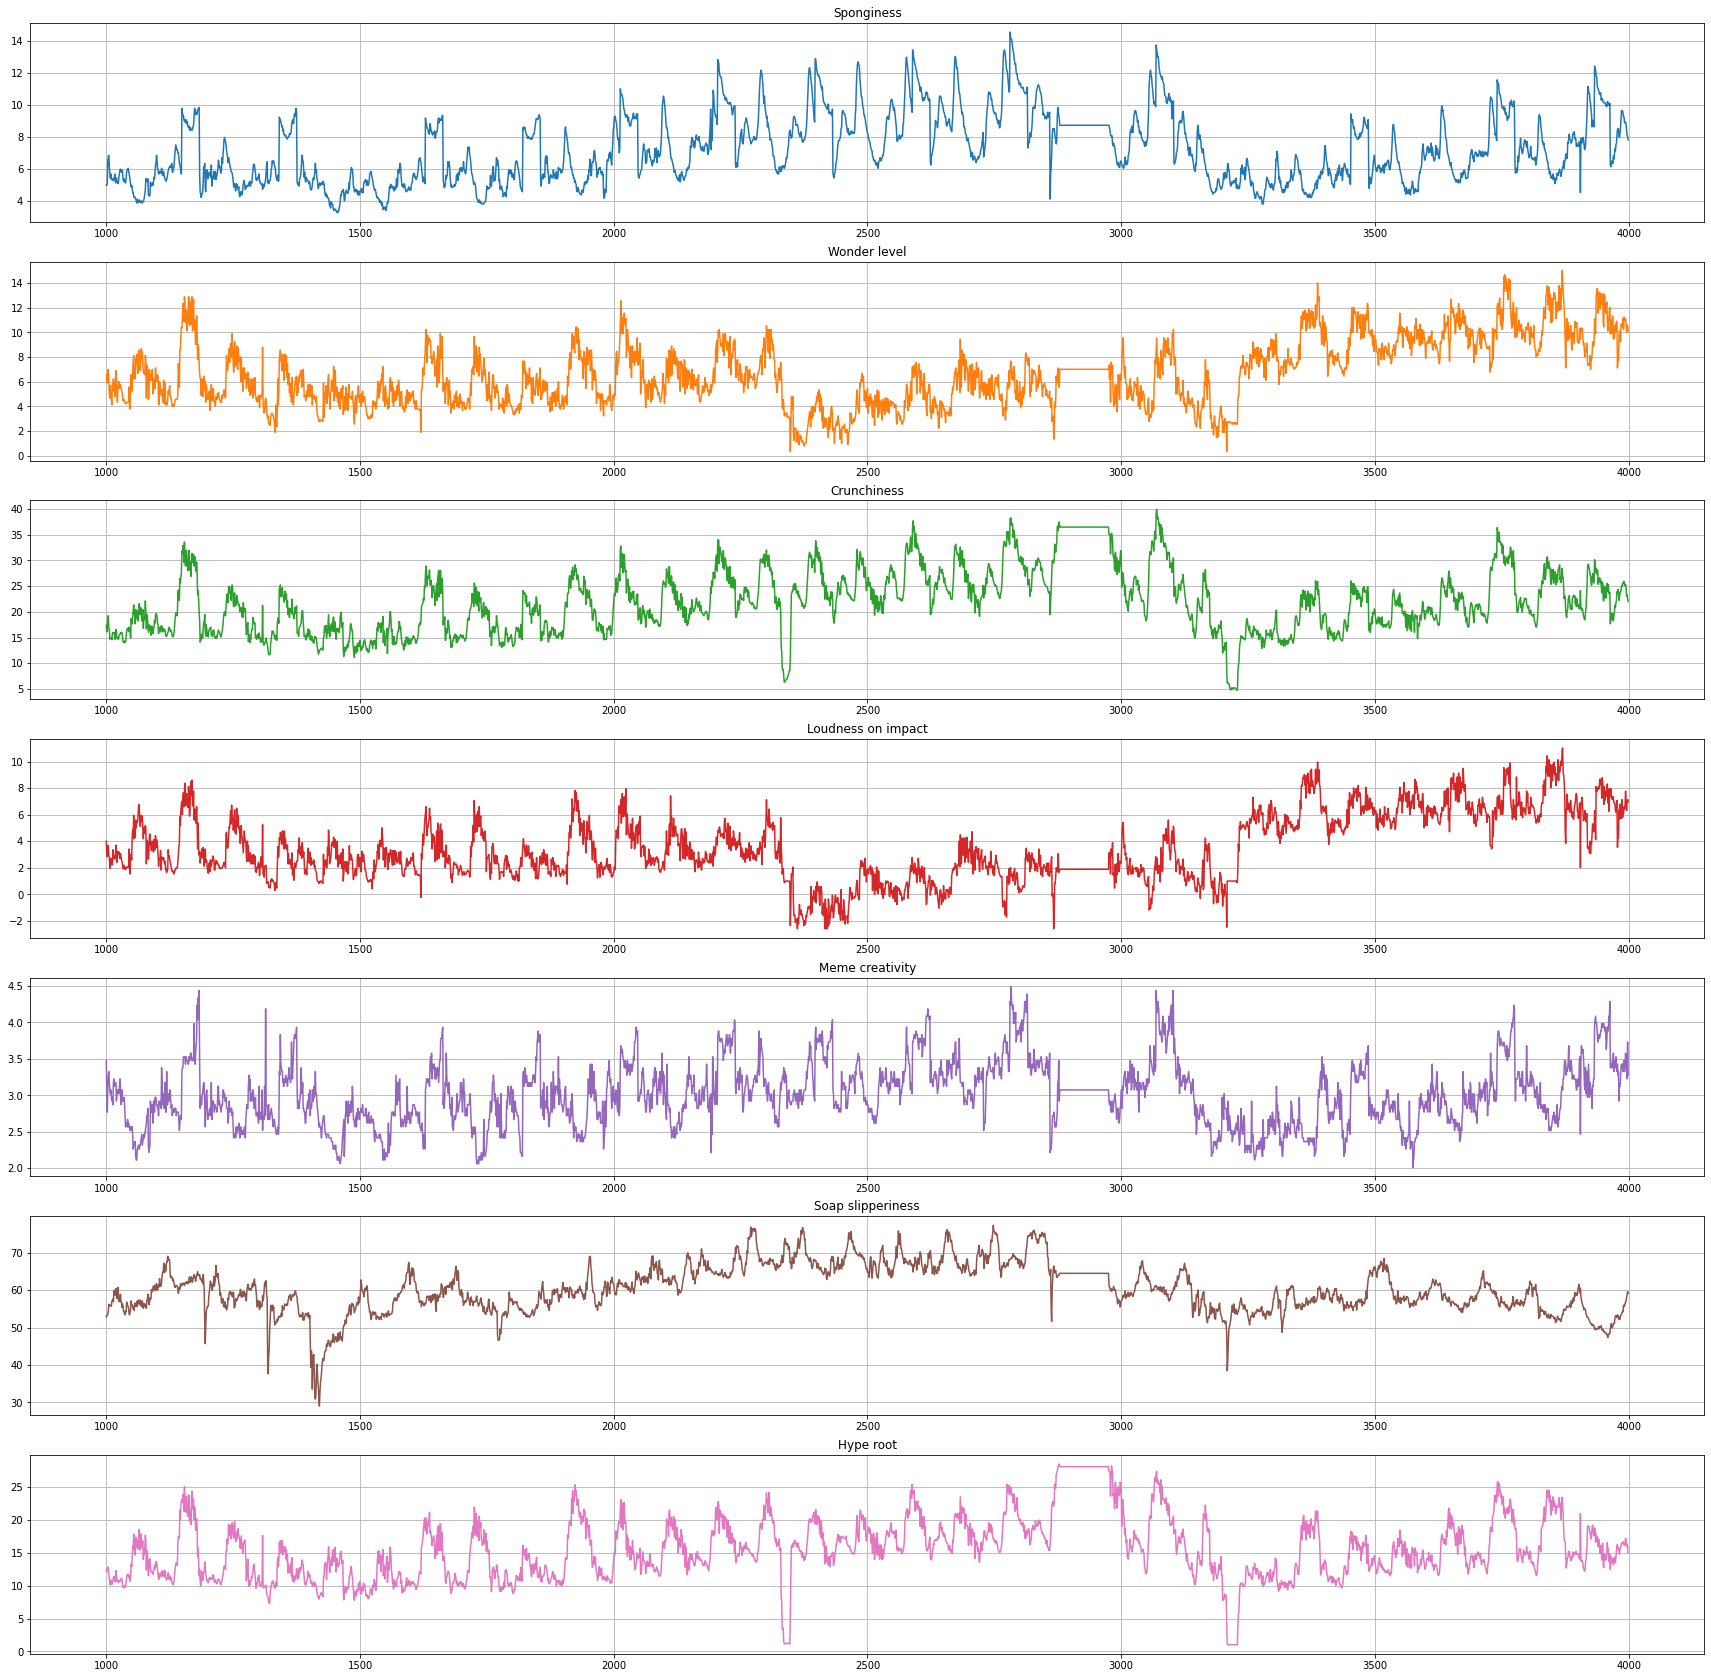
\includegraphics[width=\linewidth]{pre_processed_color.png}
        \caption{Window of the original training dataset}
        \label{fig:preprocessed_range}
    \end{figure*}
    
    \begin{figure*}[h!]
        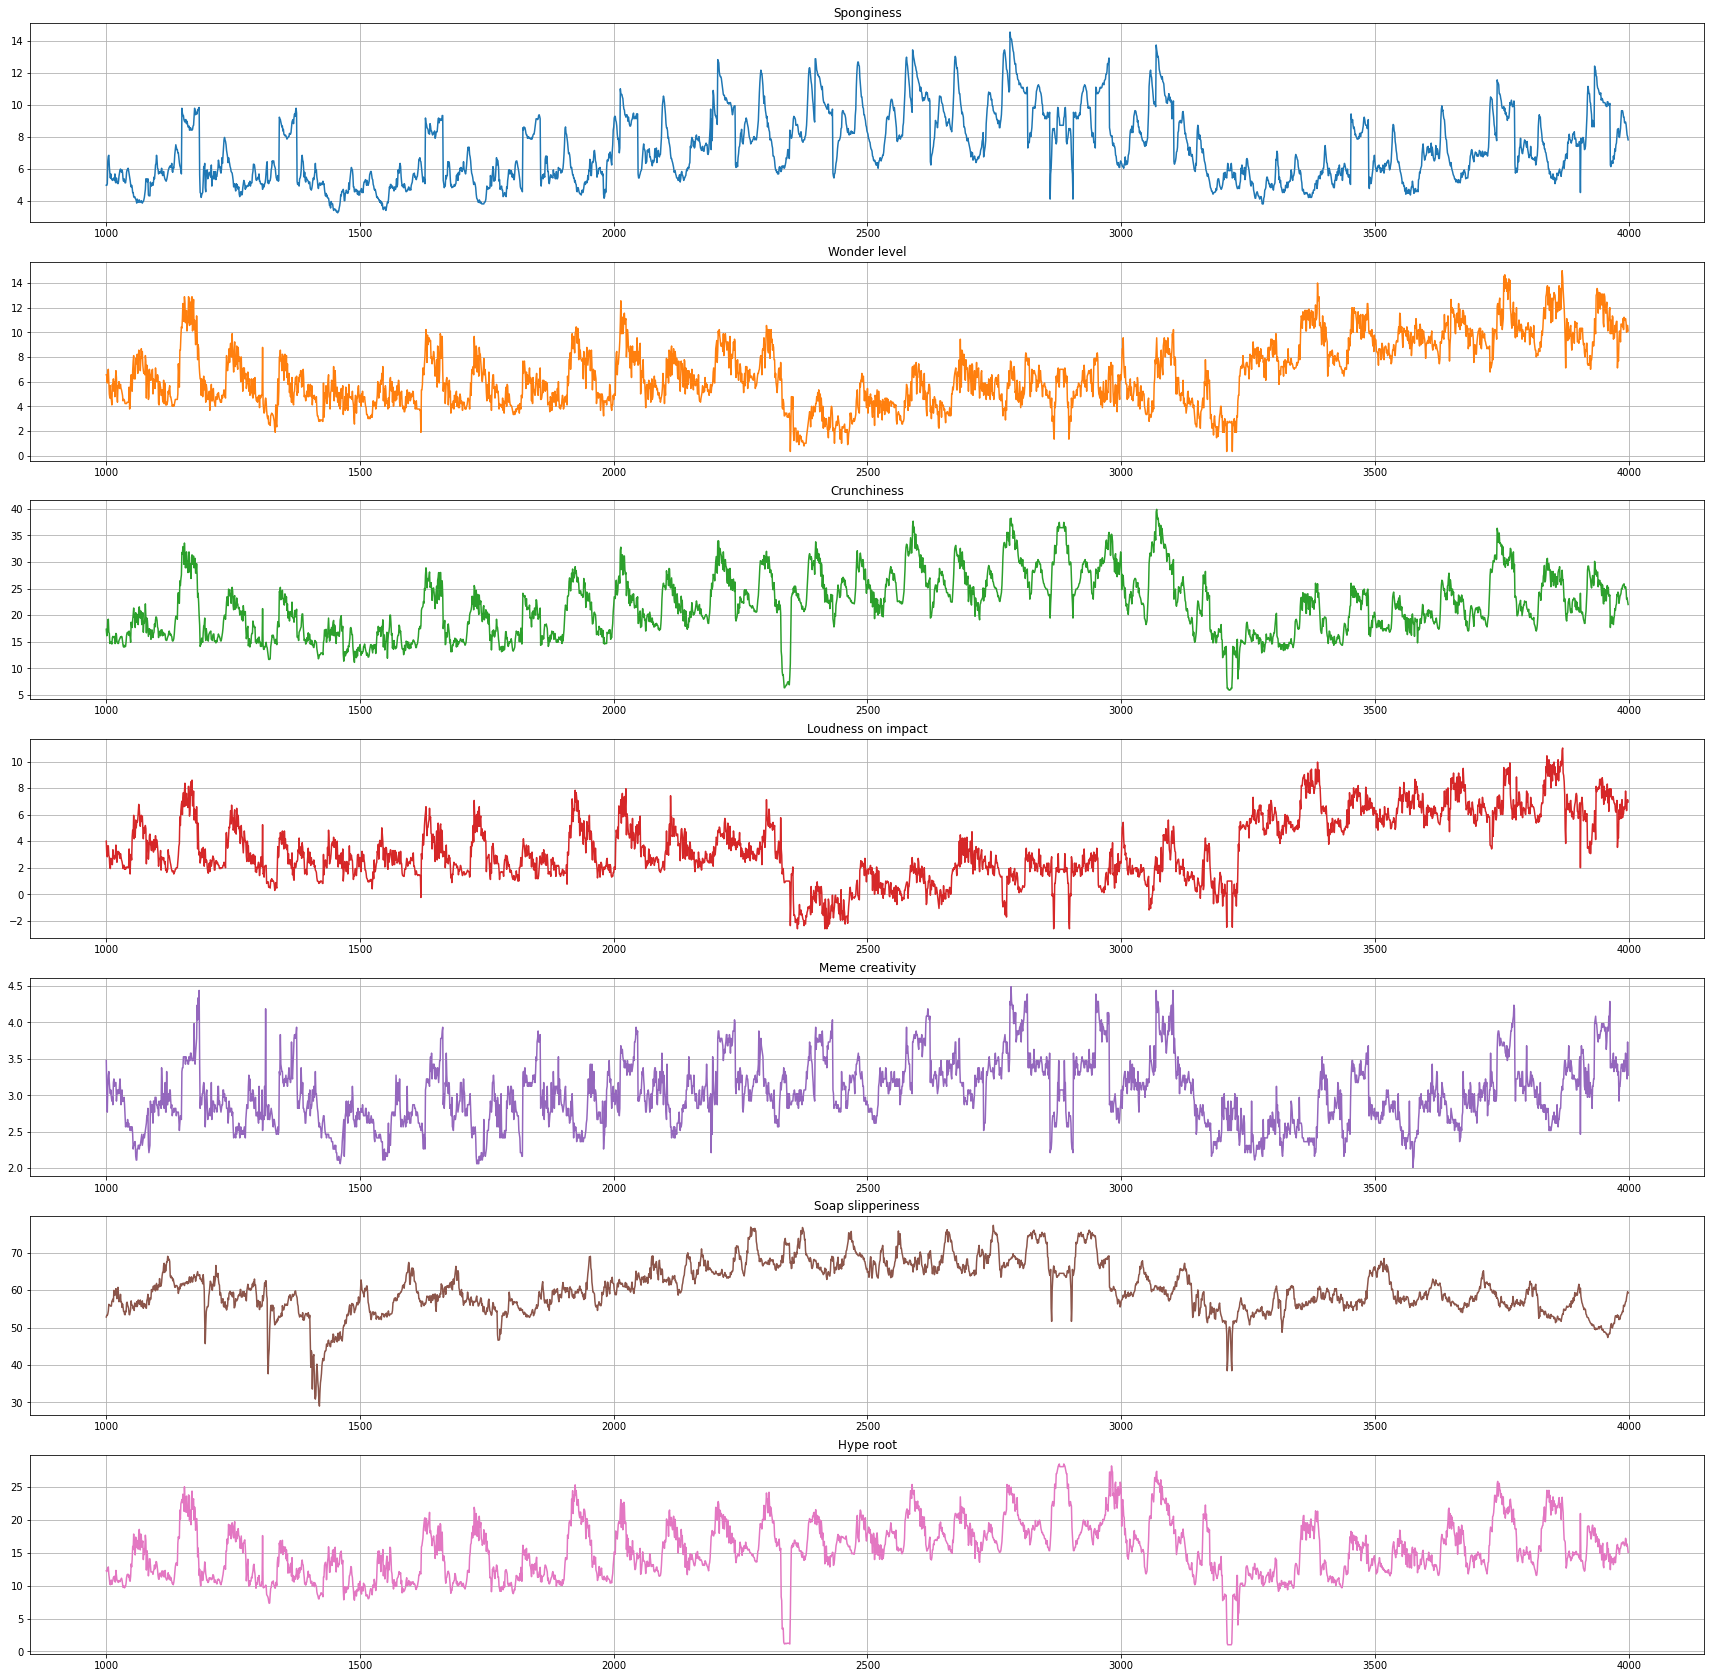
\includegraphics[width=\linewidth]{post_processed_color.png}
        \caption{Window of the training dataset after the preprocessing steps.}
        \label{fig:postprocessed_range}
    \end{figure*}
    
\end{document}